\documentclass[../main.tex]{subfiles} 
\begin{document}
\chapter{Conclusie}

\section{Beveiliging in de softwarecyclus}
kwetsbaarheden kunnen binnensluipen in elk van de softwareontwikkelingsstadia. Het is dan ook belangrijk de soorten aanvallen te kunnen onderscheiden en te weten welke tegenmaatregelen te treffen in elke situatie en fase van de ontwikkeling. Deze cursus heeft zich voornamelijk toegelegd op het implementatieniveau en af en toe het designniveau.

Het inpassen van tegenmaatregelen betekenen echter niet dat er een complete verandering nodig is in het ontwikkelingsproces. Aan de hand van \textbf{touchepoints} en \textbf{software process enrichtments} kunnen deze twee worden gecombineerd. Enkele voorbeelden zijn \textit{Cigital's touchepoints} en \textit{Microsoft's SDL}.

\section{Bedreigingsmodellering}
Het modelleren van bedreigingen is een activiteit die plaatsvindt in de beginfase van de softwareontwikkelingslevenscyclus. Het centrale doel is een goed zicht krijgen op de mogelijke kwetsbaarheden van het systeem dat wordt ontwikkeld. 

Het modelleren kan gebeuren op verschillende niveaus van abstractie:
\begin{itemize}
	\item \textbf{Systeemniveau} \\ \textit{Bv. bedreigingsmodellering van het internet e-mails systeem.}
	\item \textbf{Applicatie- of componentniveau} \\ \textit{Bv. bedreigingsmodellering van de e-mail client software.}
\end{itemize}
\noindent
Kwetsbaarheden kunnen worden onderverdeeld in categorie\"en:
\begin{itemize}
	\item \textbf{S}poofing
	\item Information \textbf{T}ampering
	\item \textbf{R}epudiation
	\item \textbf{I}nformation disclosure
	\item \textbf{D}enial of service
	\item \textbf{E}levation of privilege
\end{itemize}
Wanneer bedreigingen aan het licht worden gebracht is het belangrijk dat we een goed begrip hebben van de \textit{assets} en van de bedreigingsagent, meer bepaald wat dienst motivatie en sterkte is.

Microsoft heeft als onderdeel van het \textit{Secure Development Life Cycle} een bedreigingsmodelleringsactiviteit gedefinieerd. Aan de hand van documentatie en met gebruik van tools kunnen bedreigingen in kaart worden gebracht. Aan de hand van een voorbeeld uit dit boek zullen we het proces illustreren.

\subsection{Define Use Scenarios}
Allereerst moet gedefinieerd worden hoe het systeem gebruikt zal worden en hoe niet. Dit zorgt ervoor dat de discussie rond bedreigingsmodellering duidelijk omgrensd wordt. We vragen ons af welke scenario's binnen de strekking van het programma liggen. Bijvoorbeeld: houden we rekening met bedreigingen van interne agenten?

\subsection{List External Dependencies}
Elke applicatie steunt op infrastructurele software om correct te functioneren. Het is belangrijk om deze goed te documenteren. Nemen we als voorbeeld een winkel voor huisdieren. Deze steunt op:
\begin{multicols}{2}
\begin{itemize}
	\item Web-based client
	\item Browser
	\item Windows Server
	\item Microsoft ISS
	\item SQl Server 
	\item .NET Framework
\end{itemize}
\end{multicols}

\subsection{Define Security Assumptions}
Welke beveiligingsgaranties verwachten we van onze externe afhankelijkheden? Voor de huisdierenwinkel:
\begin{itemize}
	\item ISS en ASP.NET voorzien authenticatie
	\item Fysieke toegang tot de server is beperkt tot beheerders
	\item Configuratiebestanden worden beschermt door het besturingssysteem
\end{itemize}

\subsection{Create External Security Notes}
Documenteer beveiligingsrelevante informatie voor de gebruikers van de applicatie.
\begin{figure}[h1]
    \centering
    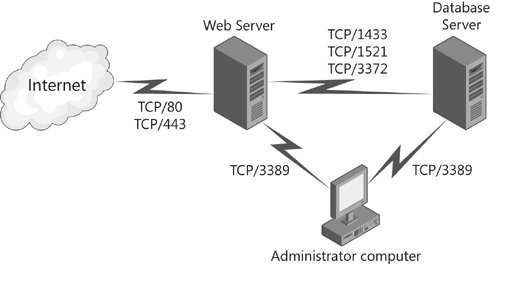
\includegraphics[width=0.6\textwidth]{../images/external_security_notes.png}
    \caption{External Security Notes}
    \label{fig:external_security_notes}
\end{figure}

\subsection{Model the Application}
Modelleer het systeem aan de hand van \textit{dataflow} diagrammen. Typisch worden volgende zaken gemodelleerd:
\begin{multicols}{2}
\begin{itemize}
	\item Externe entiteiten
	\item Processen
	\item Dataopslag
	\item Datastroom
	\item Beperkingen privileges
\end{itemize}
\end{multicols}

\begin{figure}[h!]
    \centering
    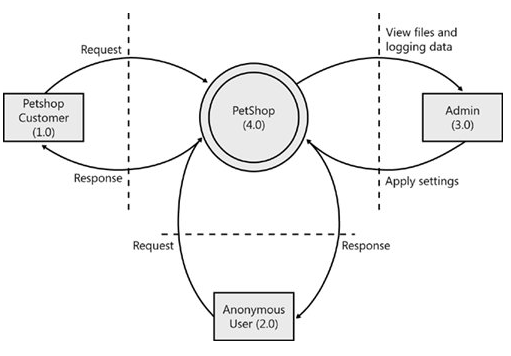
\includegraphics[width=0.6\textwidth]{../images/pet_shop_model_1.png}
    \caption{Voorbeeldmodel}
    \label{example1}
\end{figure}

\begin{figure}[h!]
    \centering
    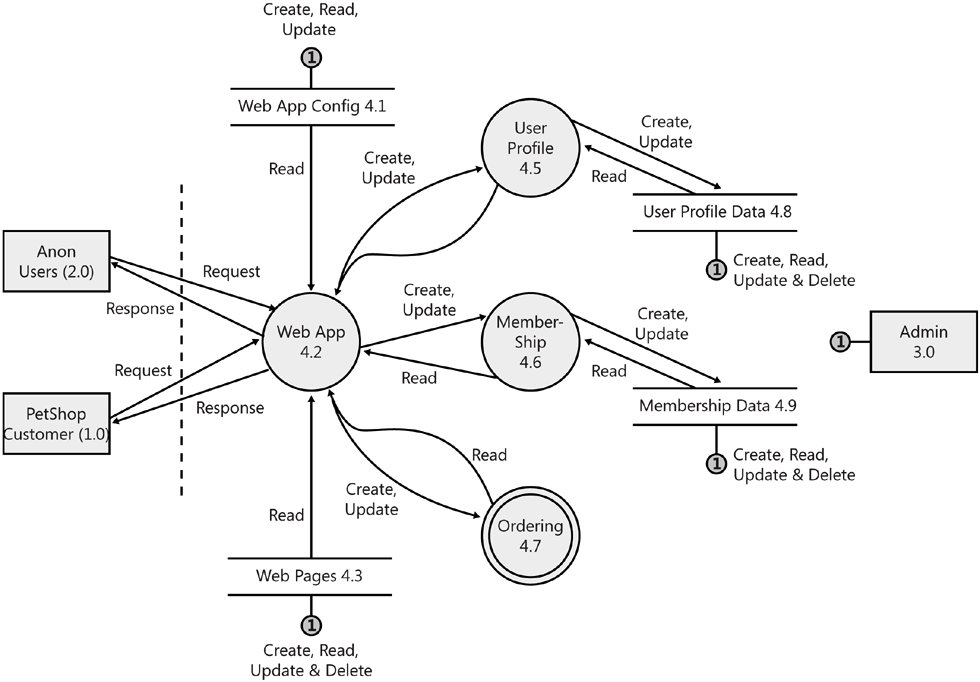
\includegraphics[width=0.8\textwidth]{../images/pet_shop_model_2.png}
    \caption{Voorbeeldmodel}
    \label{example2}
\end{figure}

\begin{figure}[h!]
    \centering
    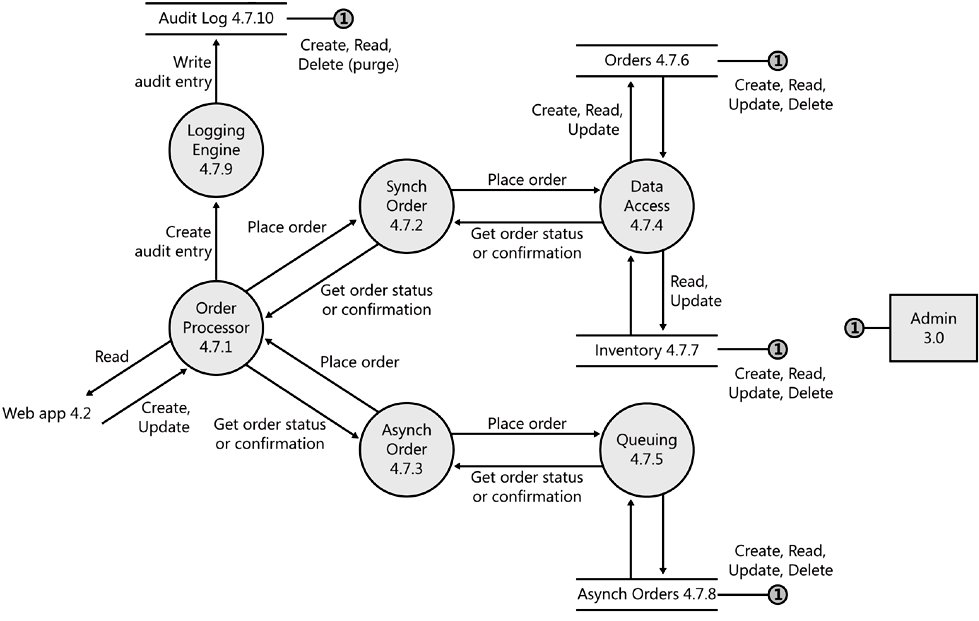
\includegraphics[width=0.8\textwidth]{../images/pet_shop_model_3.png}
    \caption{Voorbeeldmodel}
    \label{example3}
\end{figure}

\subsection{Determine Threat Types}
Microsofts proces maakt gebruikt van de  \textbf{STRIDE} bedreigingstypen. (zie eerder) 
\subsection{Identify Threats}
Alle DFD elementen worden beschouwd als \textit{assets}. Zie afbeeldinge \ref{STRIDE}.
\begin{figure}[h!]
    \centering
    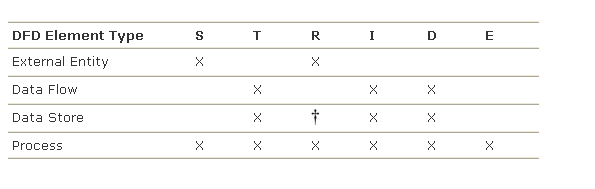
\includegraphics[width=0.8\textwidth]{../images/STRIDE.png}
    \label{STRIDE}
    \caption{DFD en STRIDE}
\end{figure}
\subsection{Determine Risk}
Subjectieve numerieke methodes om het belang te schatten (bv. DREAD) worden niet meer gebruikt. De huidige guideline zegt gebruik te maken van objectieve karakteristieken zoals 

\subsection{Plan Mitigations}
 

\section{Principes, patronen en richtlijnen}
\section{Conclusie}

\end{document}